\documentclass[times]{ettauth}
%\documentclass[times,doublespace]{ettauth}%For paper submission

\usepackage{acronym}
\usepackage{flafter}


\begin{document}
\newacro{gdp}[GDP]{Gross Domestic Product}
\newacro{citysdk}[CitySDK]{Smart City Service Development Kit and its application Pilots}
\newacro{W3C}[W3C]{World Wide Web Consortium}
\newacro{POI}[POI]{Point of Interest}
\newacro{XML}[XML]{Extensible Markup Language}
\newacro{JSON}[JSON]{JavaScript Object Notation}
\newacro{REST}[REST]{Representational State Transfer}
\newacro{HATEOAS}[HATEOAS]{Hypermedia as the Engine of Application State}
\newacro{poi}[POI]{Point of Interest}
\newacro{gis}[GIS]{Geographical Information System}
\newacro{wg}[WG]{Working Group}
\newacro{iptc}[IPTC]{International Press Telecommunications Council}
\newacro{POIs}[POIs]{Points of Interest}



\runningheads{P. Cruz \emph{et al}}{CitySDK Tourism API - Building value around open data}

\articletype{Research Article - CONFIRM}

\title{CitySDK Tourism API - Building value around open data}
\author{Pedro Cruz\affil{1},
Ricardo Lopes Pereira\affil{2}\affil{1}\corrauth\,
Andr\'e Oliveira\affil{3} and 
Geert Monsieur\affil{4}}
\address{
 \affilnum{1}Instituto Superior T\'ecnico, Avenida Rovisco Pais 1, 1049-001 Lisboa, Portugal\\
 \affilnum{2}INESC-ID, Av. Prof. Dr. Cavaco Silva, 2744-016 Porto Salvo, Portugal\\
 \affilnum{3}ISA\\
 \affilnum{4}Geert's address
}
\corraddr{E-mail: ricardo.pereira@inesc-id.pt}

\begin{abstract}
To be written latter.
\end{abstract}

\maketitle

\acresetall
\section{Introduction}

\subsection{Motivation}
The value of tourism as an economic and leisure activity.

The amount and quality of data that municipalities have in their information systems. 
Data is held not only by cities but by other entities as well.
Municipalities understand the value of this data and have gone through a multi-step process for sharing this data with tourists in order to improve their experience and attract them to the city.

First municipalities create apps for sharing data with the tourists.
Small market to recuperate investment.
Municipalities are not software houses: unable to keep up with the pace of innovation. 
They are limited in the types of applications they can provide: e.g. publishing negative opinions.

Then municipalities made data available to programmers through internal open data initiatives.
Each city uses its own format.
Programmers still have to deal with a small market.
Tourists still have difficulties finding the specific apps for each city.

\subsection{Challenges}
Common API when intersection among available data is small.
Flexibility to accommodate further usages not yet envisioned.

make way for delegation and common developer keys?


\subsection{CitySDK}
Talk about the project.

Briefly introduce the API.

This document is organised ...

This is an acronym expansion: \ac{citysdk}.
This is a test citation, to be removed later~\cite{1509968}.



\section{Related work}

\subsection{\acf{W3C} POI Working Group}
\label{section:poi-wg}
The \ac{W3C} is an international community where Member organizations, a full-time staff, and the public work together to develop Web standards. This community is led by Web inventor Tim Berners-Lee and CEO Jeffrey Jaffe. 

One of the its working groups is the \ac{W3C} POI~\cite{w3c-poi} and its mission is to develop technical specifications for the representation of \acf{POI} information on the Web. Its Core defines a generic, flexible, lightweight and extensible POI data model, and one normative syntax for the data model based on \acf{XML}. Although \ac{XML} is the primary model for this specification, other formats are also possible, such as \acf{JSON}.

The data model is shown in Figure~\ref{fig:data-model}. A brief explanation is given next.

\begin{figure*}[!ht]
\centering
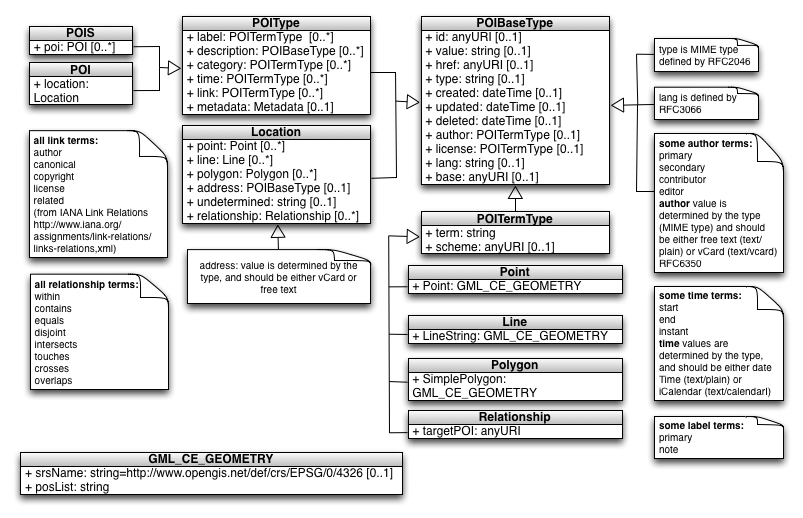
\includegraphics[width=0.8\textwidth]{images/uml}
\caption{W3C POI Core Data Model}
\label{fig:data-model}
\end{figure*}

The data model is comprised of six entities:
\begin{itemize}
\item \textbf{POIBaseType} is the common entity from which the majority of POI entities are derived. It provides basic properties related with its authorship, licensing, modification dates and identification allowing each element to carry distinct information;
\item \textbf{POITermType} is an abstract entity derived from POIBaseType and adds properties for the management of categorical descriptions, such as the ones seen in category, link, label, author, license and time properties of POIType;
\item \textbf{POIType} is an abstract entity derived from POIBaseType and adds entities for describing, labeling, categorizing and indicating the time span of a POI or group of POIs. The entity also incudes linking elements to other POIs, external web resources or metadata;
\item \textbf{Location} is of type POIBaseType and provides a flexible description of the location of a POI. A Location can be represented using geodetic coordinates for the center of the POI, line, polygon, civic address,  undetermined or bounding box (relationship element);
\item \textbf{POI} is of type POIType and adds the Location entity for describing the location of the POI;
\item Finally, \textbf{POIS} is of type POIType and can have one or more children entities of type POI.
\end{itemize}

This model is used within our API to model various types of data, as described in section~\ref{section:api-design}.

opendata

tourism and POI APIs

REST APIs?


\section{API Design}
In this section, we will describe some of the key features of the CitySDK Tourism API. We will describe the message format model, how the API is designed and some features that came along with it.

Before diving into its actual description, there are two fundamental aspects that should be mentioned. The first one, the API provides four types of data models:
\begin{itemize}
\item \textbf{Point of Interest} describes various places in a given city, ranging from monuments and museums to eating places and cultural venues; 
\item \textbf{Event} describes cultural events that happened or are about to happen in the city;
\item \textbf{Itineraries} describe a group of Points of Interest organized in such a way that describe a given topic, e.g., the life of a given person, the history of a given region or even just specific sightseeing spots;
\item \textbf{Categories/Tags} descibe a list of available categories and tagging terms for each of the aforementioned models.
\end{itemize}

Each model can also be grouped into a list of its own type, that is, each data model has a listing model where each element is either a Point of Interest, Event, Itinerary or a Category/Tag.

The second aspect is that the API is designed in a way that provides not only information about the three mentioned data models individually, but also the relationship between them and provides specific methods to retrieve specific information.

We now present the key features of the API.

\subsection{W3C POI Model in the API}
\label{section:api-design}
As mentioned before, our API provides three data models: Points of Interest, Events and Itineraries. These  models are mapped using the W3C POI Model presented in section~\ref{section:poi-wg}. We will now present how we modelled each data type.

The Points of Interest are the most easily modelled element of the API. Since the W3C POI Model is specific for this type of data we used its already specified properties to map our data model. So, the Points of Interest are mapped and described by using the POI entities directly. It should be mentioned that, since the Point of Interest is somewhat very detailed and verbose, we defined two granularities for this element: a minimal description that only includes the key essential properties and a complete model, which is the original W3C POI Data Model. The minimal model is used to map each element of a list of Points of Interest. Such list is described by the POIS entity.

The Events are modelled the same way the Points of Interest are modelled, but instead of having a Location entity completly specified, we used the relationship property of the same entity to relate a given Event to a Point of Interest. So, we have an Event completly described using the POI entity and use the relationship property to also specify and descibe the location of the event. An events list is modeled using the POIS entity, much like the Points of Interest, but it does not have a different granularity and the root name is \textit{event} instead of \textit{poi}.

\subsection{API Description}
describe the API

\subsection{Delegation}
different roles: programmer, city, museum, world wide directory.


\section{Implementation}
Talk about Lisbon's implementation



\section{Evaluation}
Answer how the challenges were met.

Evaluate the architecture from other perspectives: performance - http load balancing + delegation to multiple servers; ??



\section{Conclusions}


\acks
thank you

\bibliographystyle{wileyj}
\bibliography{references}

\end{document}


% Local IspellDict: "british"
% Local IspellPersDict: "~~/.ispell-English"

% Local Variables:
% mode: flyspell
% End:
